\chapter{Math tools}
\section{Lec 2 - A recap of SR}
We will develop some of the necessary math on this framework. \\
Let's look at the Galilean Relativity. \\
Newtonian dynamics is based on three principles
\begin{enumerate}
	\item inertia
	\item $\vec{F} = m \vec{a}$
	\item action-reaction
\end{enumerate}
The first says something like \emph{An object at rest remains at rest, and an object in motion remains in motion at constant speed and in a straight line unless acted on by an unbalanced force}. \par
The second one says:
\[
	(2): \vec{F} = 0 \implies \vec{a} = 0 \implies (1)
\]

So, it seems the first principle is contained by the second, but we know that $\vec{F} = m \vec{a} $ is valid only in Inertial Frames (IF). \par
\paragraph{Galilean Relativity:} all the laws of \emph{mechanics} take the same form in every IF. (You can not distinguish two IF just by doing experiments.) \par
\begin{figure}
\begin{minipage}[t]{0.4\textwidth}
    \vspace*{0pt} 
    \centering
    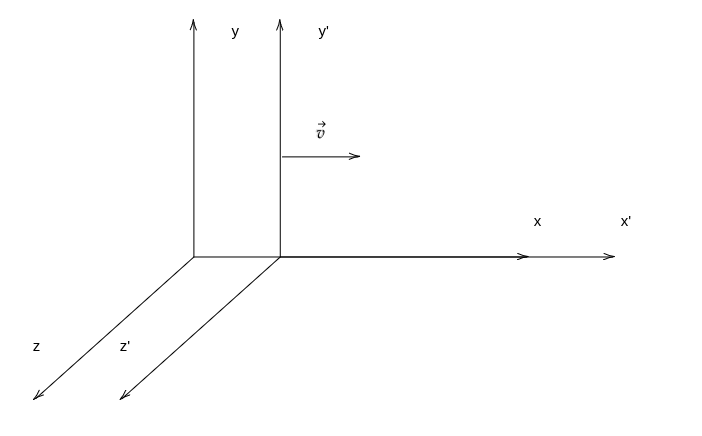
\includegraphics[width=\linewidth]{imm/galileianboost.png} 
    %\caption{G. Boost}
\end{minipage}

\end{figure}
\begin{minipage}[t]{0.4\textwidth}
    \vspace*{0pt}
    $
    \begin{cases}
    x' = x - vt \\
    y' = y \\
    z' = z \\
    t' = t
    \end{cases}$ \par
      $t = t' = 0 \implies O = O'$
\end{minipage} 
\bigskip

Taking the first derivative:
\begin{equation}
\begin{cases}
v_{x}' = v_{x} - v \\
v_{y}' = v_{y} \\
v_{z}' = v_{z} \\
\end{cases} \text{and for the second derivative: } \\
\begin{cases}
a_{x}' = a_{x} \\
a_{y}' = a_{y}\\
a_{z}' = a_{z}
\end{cases} \implies \vec{a}' = \vec{a}
\end{equation}
so also $\vec{F}' = \vec{F}$. And if \emph{m} is independent on the frame, we got
\begin{equation}
\vec{F}'=m \vec{a}' = \vec{F} = m \vec{a}
\end{equation}
\bigskip

Then there are Maxwell equations, people thanks to them find that EM-waves propagates with speed \emph{c} in the void. \par
But they found also that these equations were not invariant in Galilean Boosts. \par
Things started to go better when the idea of a preferred IF was ditched and Einstein decided to use Lorentz Transformations.\par

There are two postulates: \par
\begin{itemize}
	\item \emph{Relativity principle}: same as before but with \emph{physics} instead of \emph{mechanics}. \textbf{All the laws of physics ...}
	\item \emph{Speed of light}: in every IF, light propagates with constant speed, \emph{c}.
\end{itemize}
So we see that Galilean transformation become inconsistent with this, meanwhile stays valid for $\vec{v} \ll \vec{c}$.\par
As mentioned before, updated version of G. Boosts are Lorentz transformations (or Lorentz Boosts.)
\begin{equation}
\begin{cases}
	x' = \frac{x-vt}{\sqrt{1-(\frac{v}{c})^{2}}} \\
	y' = y \\
	z' = z \\
	t' = \frac{t- \frac{vx}{c^{2}}}{\sqrt{1-(\frac{v}{c})^{2}}}
\end{cases}
\end{equation}

To ensure the L.T. Is consistent we can perform three checks:
\begin{itemize}
	\item $v \ll c$
	\item v = 0
	\item dimensional check
\end{itemize}
People use a notation to make the L.T. easier to write: $\gamma(v) \equiv \frac{1}{\sqrt{1-(\frac{v}{c})^{2}}} $, so it becomes
\begin{equation}
\begin{cases}
x' = \gamma (x-vt) \\
y' = y \\
z' = z \\
t' = \gamma (t- \frac{vx}{c^{2}})
\end{cases}
\end{equation}

What happens to the transformation of velocity is: (v is fixed) 
\begin{equation}
\begin{cases}
dx' = \gamma(dx -vdt) \\
dy' = dy \\
dz' = dz \\
dt' = \gamma \left(dt - \frac{v dx}{c^{2}}\right)
\end{cases}
\end{equation}
 so 
\begin{equation}
\begin{cases}
 v_{x}' = \frac{dx'}{dt'} \\
 v_{y}' = \frac{dy'}{dt} = \frac{dy}{\gamma \left(dt - \frac{vdx}{c^{2}}\right)} = \frac{v_{y}}{\gamma \left(1- \frac{v v_{x}}{c^{2}}\right)} \\
v_{z}' = \frac{dz'}{dt} = ...
\end{cases}
\end{equation}
So we see that space-time changes also along other axes.\par

Now let's talk about space-time and its parts.

\paragraph{Space-time} space-time is a manifold. For now it is a collection of (t,x,y,z), four dimensional set of all the possible values of the coordinates.
\paragraph{Event} a point of space-time.
\paragraph{World line} path of a particle in space-time.

\begin{figure}
\centering
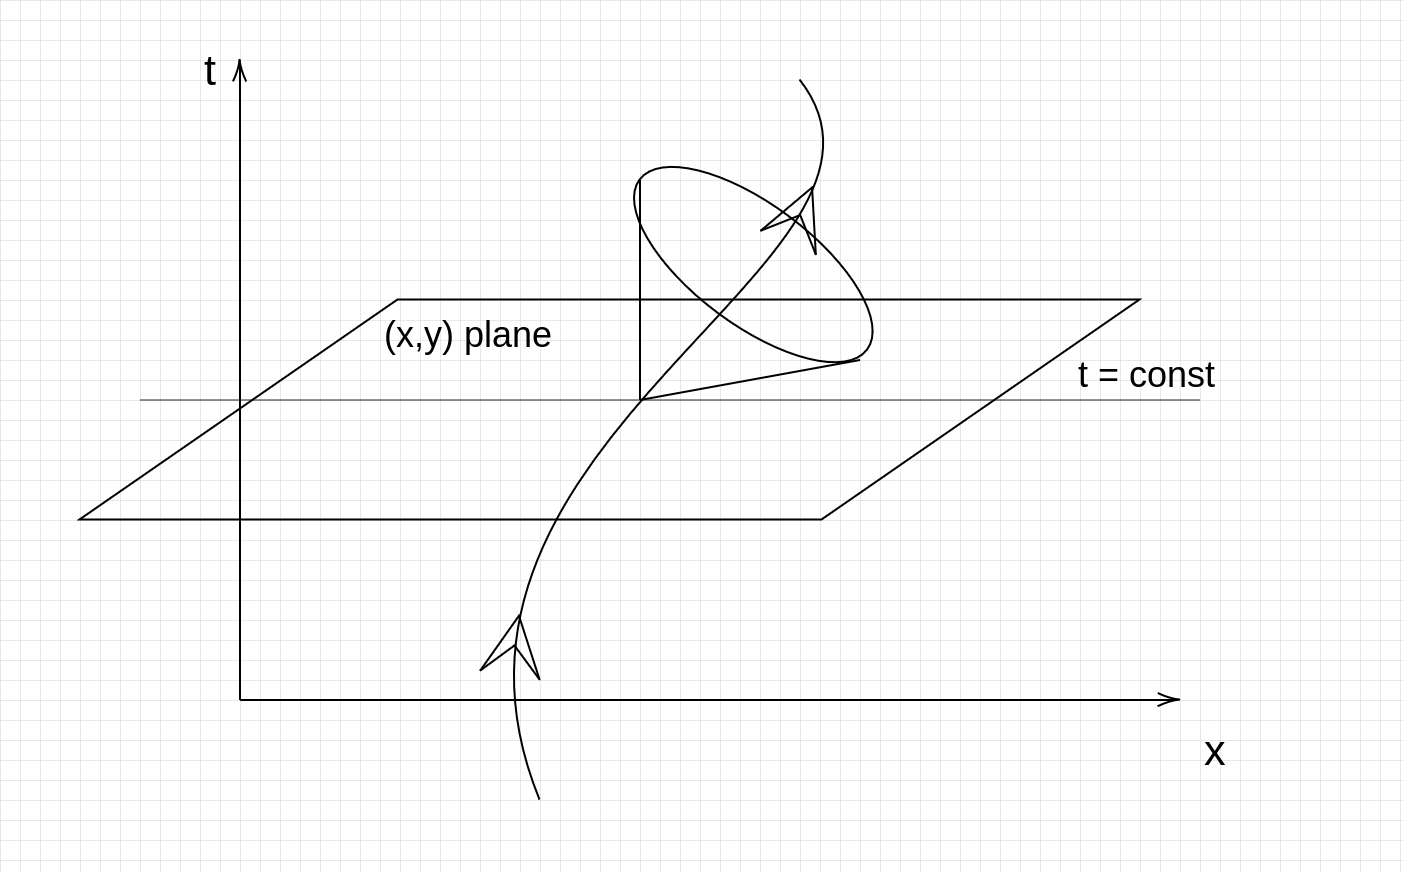
\includegraphics[width=\linewidth]{imm/WLLC.png}
\caption{LL of a particle which moves forward in time, we see also a light cone}
\label{mm:WLLC}
\end{figure}

There is no notion of absolute time anymore, because now it is dependent on the frame. 
Regarding the light-cone, after the event on the ( x,y ) plane, the particle can move \emph{only} inside the light-cone, in the appropriate direction (time forward).
Now let's talk about \textbf{Clock Synchronization.} \par
It is kinda easy if in in IF. In GR it is quite subtle instead. \par

\paragraph{Example:} Be me in Origin of a RF watching my clock (A). How to define \emph{t} at another generic location (B)??

\begin{figure}
\centering
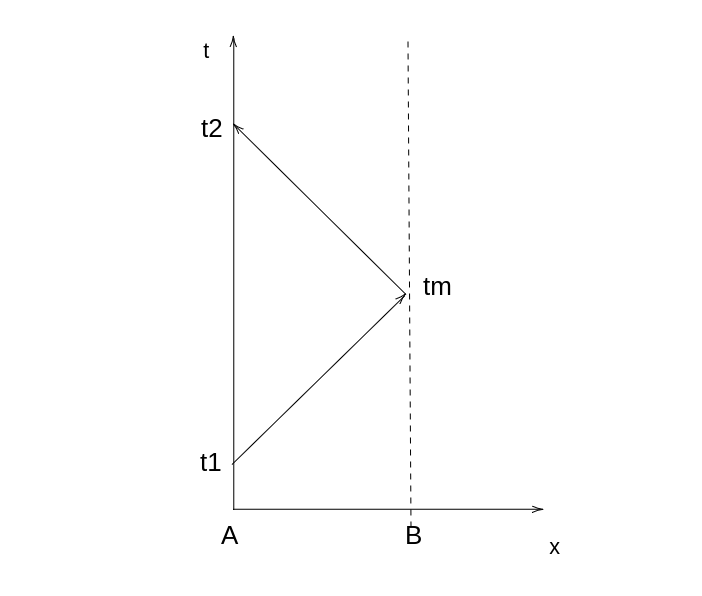
\includegraphics[width=\linewidth]{imm/segnale.png}
\caption{Reception and send of the signal}
\label{imm:segnale.png}
\end{figure}

I send a light ray at time \emph{t\textsubscript{1}} to B. I get the answer on \emph{t\textsubscript{2}}. There is symmetry between the two trajectories so \[
t_{m} = \frac{ t_{1} + t_{2} }{2}. 
\]
I say to my friend on B: "set your clock to t\textsubscript{m} when you receive the signal."
So, following this methodology, each point could have its own clock.

\paragraph{Proper time:} How to define proper time? \\
\emph{t} is the time coordinate. Let's introduce the metric tensor:
\begin{equation}
	\text{the Minkowski metric tensor: } \eta_{\mu \nu } = \begin{pmatrix}
	-1 & 0 & 0 & 0 \\
	0 & 1 & 0 & 0 \\
	0 & 0 & 1 & 0 \\
	0 & 0 & 0 & 1
	\end{pmatrix} 		
\end{equation}
for a Lorentz Transformation if I have 2 events E,F.
\begin{gather*}
	\text{Frame 1: } x_{F}^{\mu } = \left( t_{F}, x_{F}, y_{F}, z_{F} \right)\\
	x_{E} = \left( ... \right) \\
	\text{Frame 2: } x_{F}^{\mu' } = \left( t_{F'}, x_{F'}, y_{F'}, z_{F'} \right) \\
	x_{E}^{\mu' } = \left( ... \right)	 
\end{gather*}
same events in 2 different frames. \\
A Lorentz Transformation cornets these two events.

Be $\Delta s^{2}$ the Lorentz Invariant separation between E-F.
\begin{gather*}
\Delta s^{2} = -c \left( t_{F}-t_{E} \right)^{2} + \left( x_{F}- x_{E} \right)^{2} + \left( y_{F}-y_{E} \right)^{2} + \left( z_{F}-z_{E} \right)^{2} =\\
= -c (t_{F'}-t_{E'})^{2}  + (x_{F'}- x_{E'})^{2}  + (y_{F'}-y_{E'})^{2}  + (z_{F'}-z_{E'})^{2} \\
\Delta s^{2} = \eta_{\mu \nu } \Delta x^{\mu } \Delta x^{\nu } \\
\text{From this point we set } c = 1 \text{ just a rescaling} \\
\text{we have defined } \Delta x^{\mu } \equiv x_{F}^{\mu} - x_{F}^{\mu }, \text{with } \mu = 0,1,2,3.
\end{gather*}

So, repeating for clarity, the Lorentz Invariant separation is
\begin{equation}
\Delta s^{2} = \eta_{\mu  \nu } \Delta x^{\mu } x^{\nu } = \eta_{\mu'\nu'} \Delta x^{\mu '} \Delta x^{\nu'}
\end{equation}
Minkowski metric tensor does not change form if we change coordinates (Cartesian coordinates, meanwhile if we use like polar ones it changes for obvious reasons.) \par

if 
\begin{align*}
	\Delta s^{2} & > 0 \text{space-like separation} \\
		     &< \text{time-like, (it could be an actual LL for a massive particle)} \\
		     &= \text{light-like or null}
\end{align*}

Now we can define the \emph{proper time} as
\begin{equation}
	\Delta \tau^{2} \equiv - \Delta s^{2} \text{ or } \Delta \tau^{2} = - \eta_{\mu  \nu }\Delta x^{\mu } \Delta x^{\nu }
\end{equation}
So, if the proper time is \emph{positive} it is time-like.

If the segment \textbf{EF} marks the begin and end of the trajectory of a massive particle, $\Delta  \tau $, proper time, is the time elapsed on a clock sitting on a RF that moves with constant speed between E and F.
\\
Int the moving frame $\Delta \tau = \Delta t_{*}$ where \emph{t\textsubscript{*}} is the time coordinate of the moving frame. 
In a frame where I'm at rest this is how $\Delta t^{2}$ changes:
\begin{equation}
\Delta  \tau^{2} = + \Delta t^{2} - \Delta x^{2} - \Delta y^{2}- \Delta z^{2}.
\end{equation}
